\section{Задача 2.16}
\subsection{Задание:}
Построить два различных скелетных разложения матрицы $ A $.
\\[1em]
$
	A = \begin{pmatrix}
		-3 & 5 & 4 & -17 & -7 & -11 \\
		1 & 3 & -4 & 1 & -17 & 9 \\
		2 & 0 & -8 & 8 & -16 & 18 \\
		-4 & -6 & 2 & -10 & 22 & -8
	\end{pmatrix}
$
\subsection{Решение:}
Определим линейно независимые строки матрицы $ A $:
\\
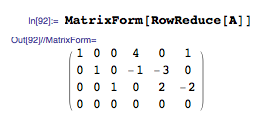
\includegraphics[scale=0.6]{task/2_16/screen1.png}
\\
Первые три строки матрицы $ A $ линейно независимы. Построим матрицу $ C $:
\\[1em]
$
	C =
	\begin{pmatrix}
		-3 & 5 & 4 & -17 & -7 & -11 \\
		1 & 3 & -4 & 1 & -17 & 9 \\
		2 & 0 & -8 & 8 & -16 & 18 \\
	\end{pmatrix}
$
\\[1em]
Из $ A = BC $ найдём матрицу $ B $:
\\[1em]
$
	B = AC^{+} =
	\begin{pmatrix}
		1 & 0 & 0 \\
		0 & 1 & 0 \\
		0 & 0 & 1 \\
		\frac{7}{4} & -\frac{59}{12} & \frac{37}{12}
	\end{pmatrix}
$
Выполним компьютерную проверку разложения в среде Wolfram Mathematica:
\\
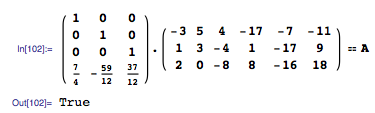
\includegraphics[scale=0.6]{task/2_16/screen2.png}
\\[1em]
Построим второе скелетное разложение $ A $:
\\
Определим линейно независимые столбцы:
\\
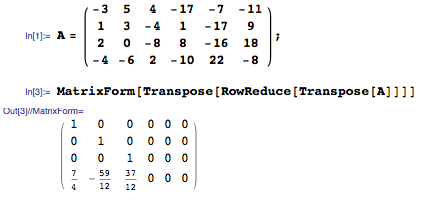
\includegraphics[scale=0.6]{task/2_16/screen3.png}
\\
Видно что первые три столбца матрицы линейно независимы. Составим матрицу $ B $:
\\[1em]
$
	B =
	\begin{pmatrix}
		-3 & 5 & 4 \\
		1 & 3 & -4 \\
		2 & 0 & -8 \\
		-4 & -6 & 2 \\
	\end{pmatrix}
$
\\[1em]
Найдём матрицу $ C $ из $ A = BC $:
\\[1em]
$
	C = B^{+}A =
	\begin{pmatrix}
		1 & 0 & 0 & 4 & 0 & 1 \\
		0 & 1 & 0 & -1 & -3 & 0 \\
		0 & 0 & 1 & 0 & 2 & -2 \\
	\end{pmatrix}
$
\\[1em]
Выполним компьютерную проверку в среде Wolfram Mathematica:
\\
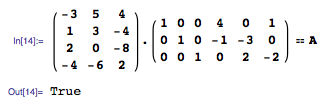
\includegraphics[scale=0.6]{task/2_16/screen4.png}
\subsection{Вывод:}
Мы построили два скелетных разложения матрицы $ A $.
